%!TEX root = draft.tex
% \vspace{-10pt}
\section{Modeling Local Mixing Patterns}
\label{subsec:LocalMixing}

The global assortativity coefficient quantifies
% the level of homophily or heterophily in an attributed network. It sheds light
% on
the average propensity of links to occur between similar nodes.
%  by capturing
% the attribute mixing pattern across the entire network.
However, global assortativity is not a representative summary statistic of
heterogeneous mixing patterns observed in large-scale networks~\cite{peel2018multiscale}.
Furthermore, it does not quantify anomalous mixing patterns and fails to measure how mixing varies across a network.

We use local assortativity~\cite{peel2018multiscale} to measure varying
mixing patterns in an attributed network $G=(V,E,B)$ with attribute values $B=\{b_1...b_l\}$.
Unlike global assortativity that counts all edges between similar nodes, local assortativity
of node $i$, $r_l(i)$, captures mixing pattern in the local neighborhood of node
$i$ by using a locality biased weight distribution $w_i$. The distribution
$w_i$ reweighs edges between similar nodes based on how local they are to
node $i$. As~\citet{peel2018multiscale} indicate, there are multiple ways
to define $w_i$, and we define $w_i(j) = \sfrac{1}{|N(i)|}$ for all $j \in N(i)$, as this allows for a highly efficient local assortativity calculation.

% The distribution $w_i$ reweighs edges between similar nodes
% based on how local they are to node $i$. Peel et al. \cite{peel2018multiscale} prescribe a
% personalized pagerank weight distribution, which is prohibitively expensive to compute for
% all nodes in large graphs; Large network datasets necessitate efficient weighting schemes.
% Therefore, we define $w_i$ as a uniform distribution
% over $N(i)$, the set of nodes that are at most 1 hop away from node $i$.

% reintroduce only if there is room.
% More formally, the local assortativity coefficient $r_l(i)$ of node $i$, with outdegree $m(i)$ and
% attribute value $b(i)$ is defined as follows:
% \vspace{-1mm}
% \begin{align*}
% 	\scriptsize r_l(i) = \frac{\overbrace{\frac{1}{|N(i)|}\sum\limits_{j \in N(i)}^{m(j) > 0} \sum_{k \in V} \frac{\mathcal{I}\{(j,k) \in E \wedge b(j)=b(k)\}}{m(i)} }^{\texttt{obs}}-\overbrace{\sum_{b \in B} e_{b}\cdot e_{b}}^{\texttt{rnd}}}{\underbrace{1}_{\max(\texttt{obs})}-\underbrace{\sum_{b \in B} e_{b} \cdot e_{b}}_\texttt{rnd}}
% \end{align*}
% Intuitively, $r_l(i)$ compares the observed fraction of edges between similar nodes
% in the local neighborhood of node $i$ (\texttt{obs}) to the expected fraction
% if the edges are randomly rewired (\texttt{rnd}).

As shown in~\Cref{fig:local_atty}, local assortativity distributions
of \texttt{ACL}, \texttt{APS} and \texttt{Patents} reveal anomalous, skewed
and heterophilic local mixing patterns that are not inferred via global assortativity.

\begin{figure}[h]
	\centering
	\vspace{-9pt}
	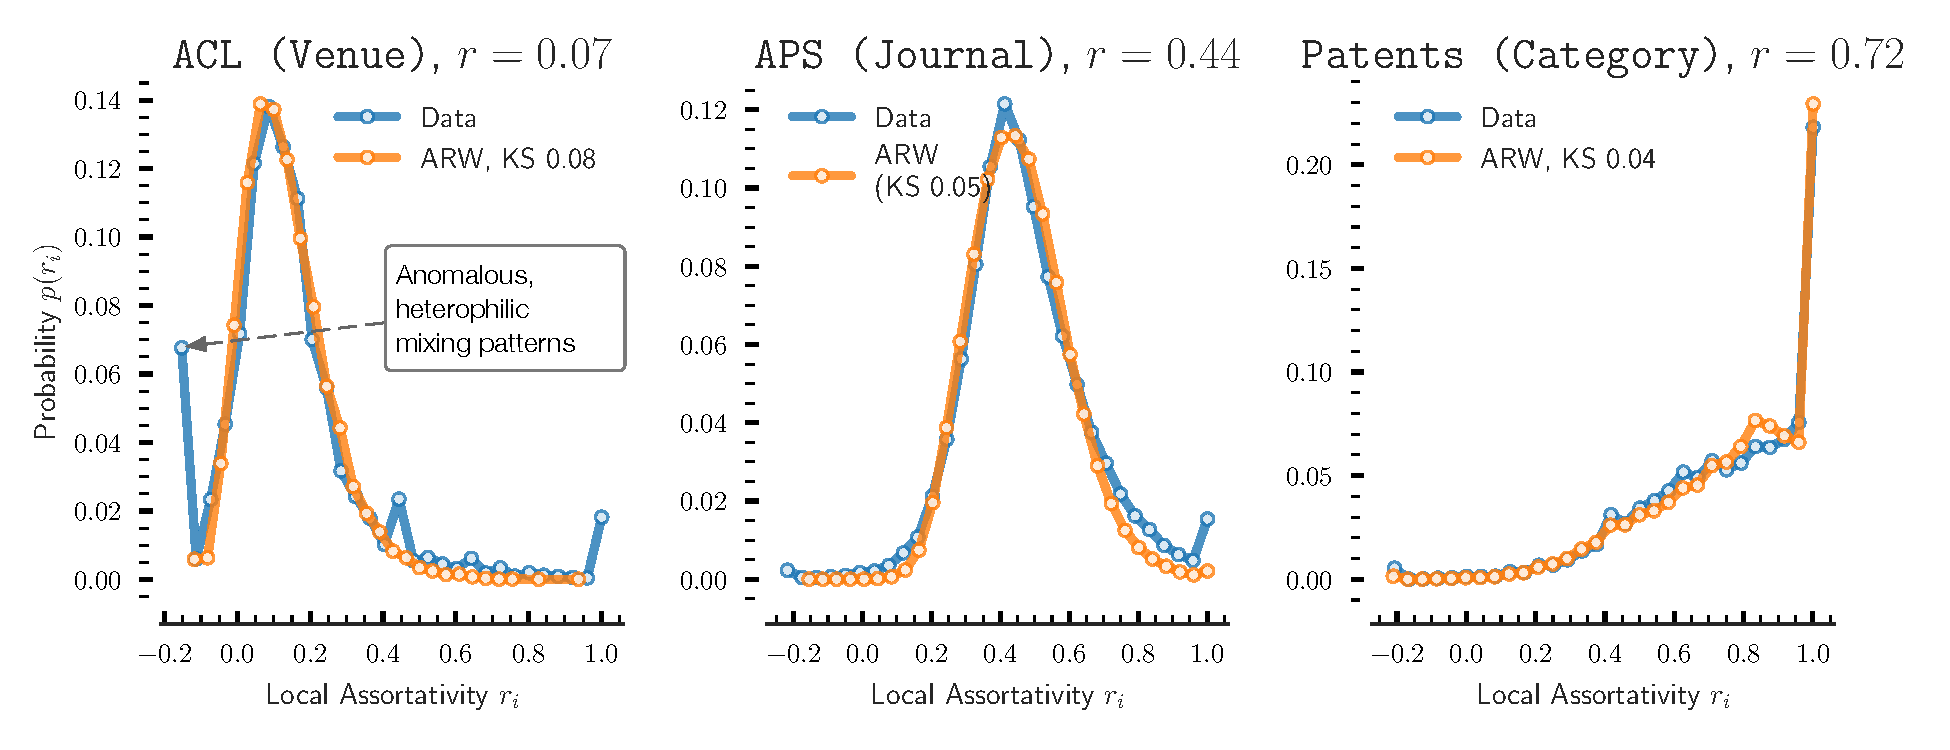
\includegraphics[width=\linewidth]{local_atty_dist3f}
	\caption{Local assortativity distributions of attributed networks \texttt{ACL}, \texttt{APS}
		and \texttt{Patents} reveal anomalous, skewed and even heterophilic local mixing patterns.
		\texttt{ARW} accurately preserves local assortativity, but does not account for anomalous mixing patterns.}
	\label{fig:local_atty}
	\vspace{-8pt}
\end{figure}

\texttt{ARW} can preserve
diverse local assortativity distributions with high accuracy even though nodes
share the same attribute preference parameter $p_a$. This is because, in addition
to sample attributes conditioned on time, \texttt{ARW}
incorporates multiple sources of stochasticity through its edge formation
mechanism. As a result, incoming nodes with fixed homophilic preferences can end
up having variable local assortativity by (a) selecting a seed node in a region
with too few (or too many) similar nodes or (b) exhausting all its links before
visiting similar (or dissimilar) nodes.
\texttt{ARW} is not expressive enough to model anomalous
mixing patterns. Mechanisms such as sampling $p_a$ from a mixture of
Bernoullis are necessary to account for anomalous mixing patterns.
